% chapters/chapter06.tex
\chapter{Le regole del convitto}

Luca è a pochi metri da Giovanni e ha un vantaggio evidente: infatti, ci vede.

\par\medskip
Ipparchia non ha dato segni di nervosismo, ma il secondo cane mostra di essere pronto a reagire ad un'aggressione.

\par\medskip
«Allora ferma questo colpo!» grida, e si lancia verso Giovanni brandendo un bastone sopra la testa.

\par\medskip
Raggiunge il \textbf{MA-AI} per colpirlo, ma a quel punto i suoi movimenti si fanno lenti. Giovanni abbassa di poco la testa, alza le mani e rapidamente blocca il bastone.

\par\medskip
Osservandolo dall'esterno, sembra che stia pregando. Ha le mani chiuse, palmo contro palmo, e in mezzo c'è il bastone. Una contromossa ninja.

\par\medskip
\begin{center}
  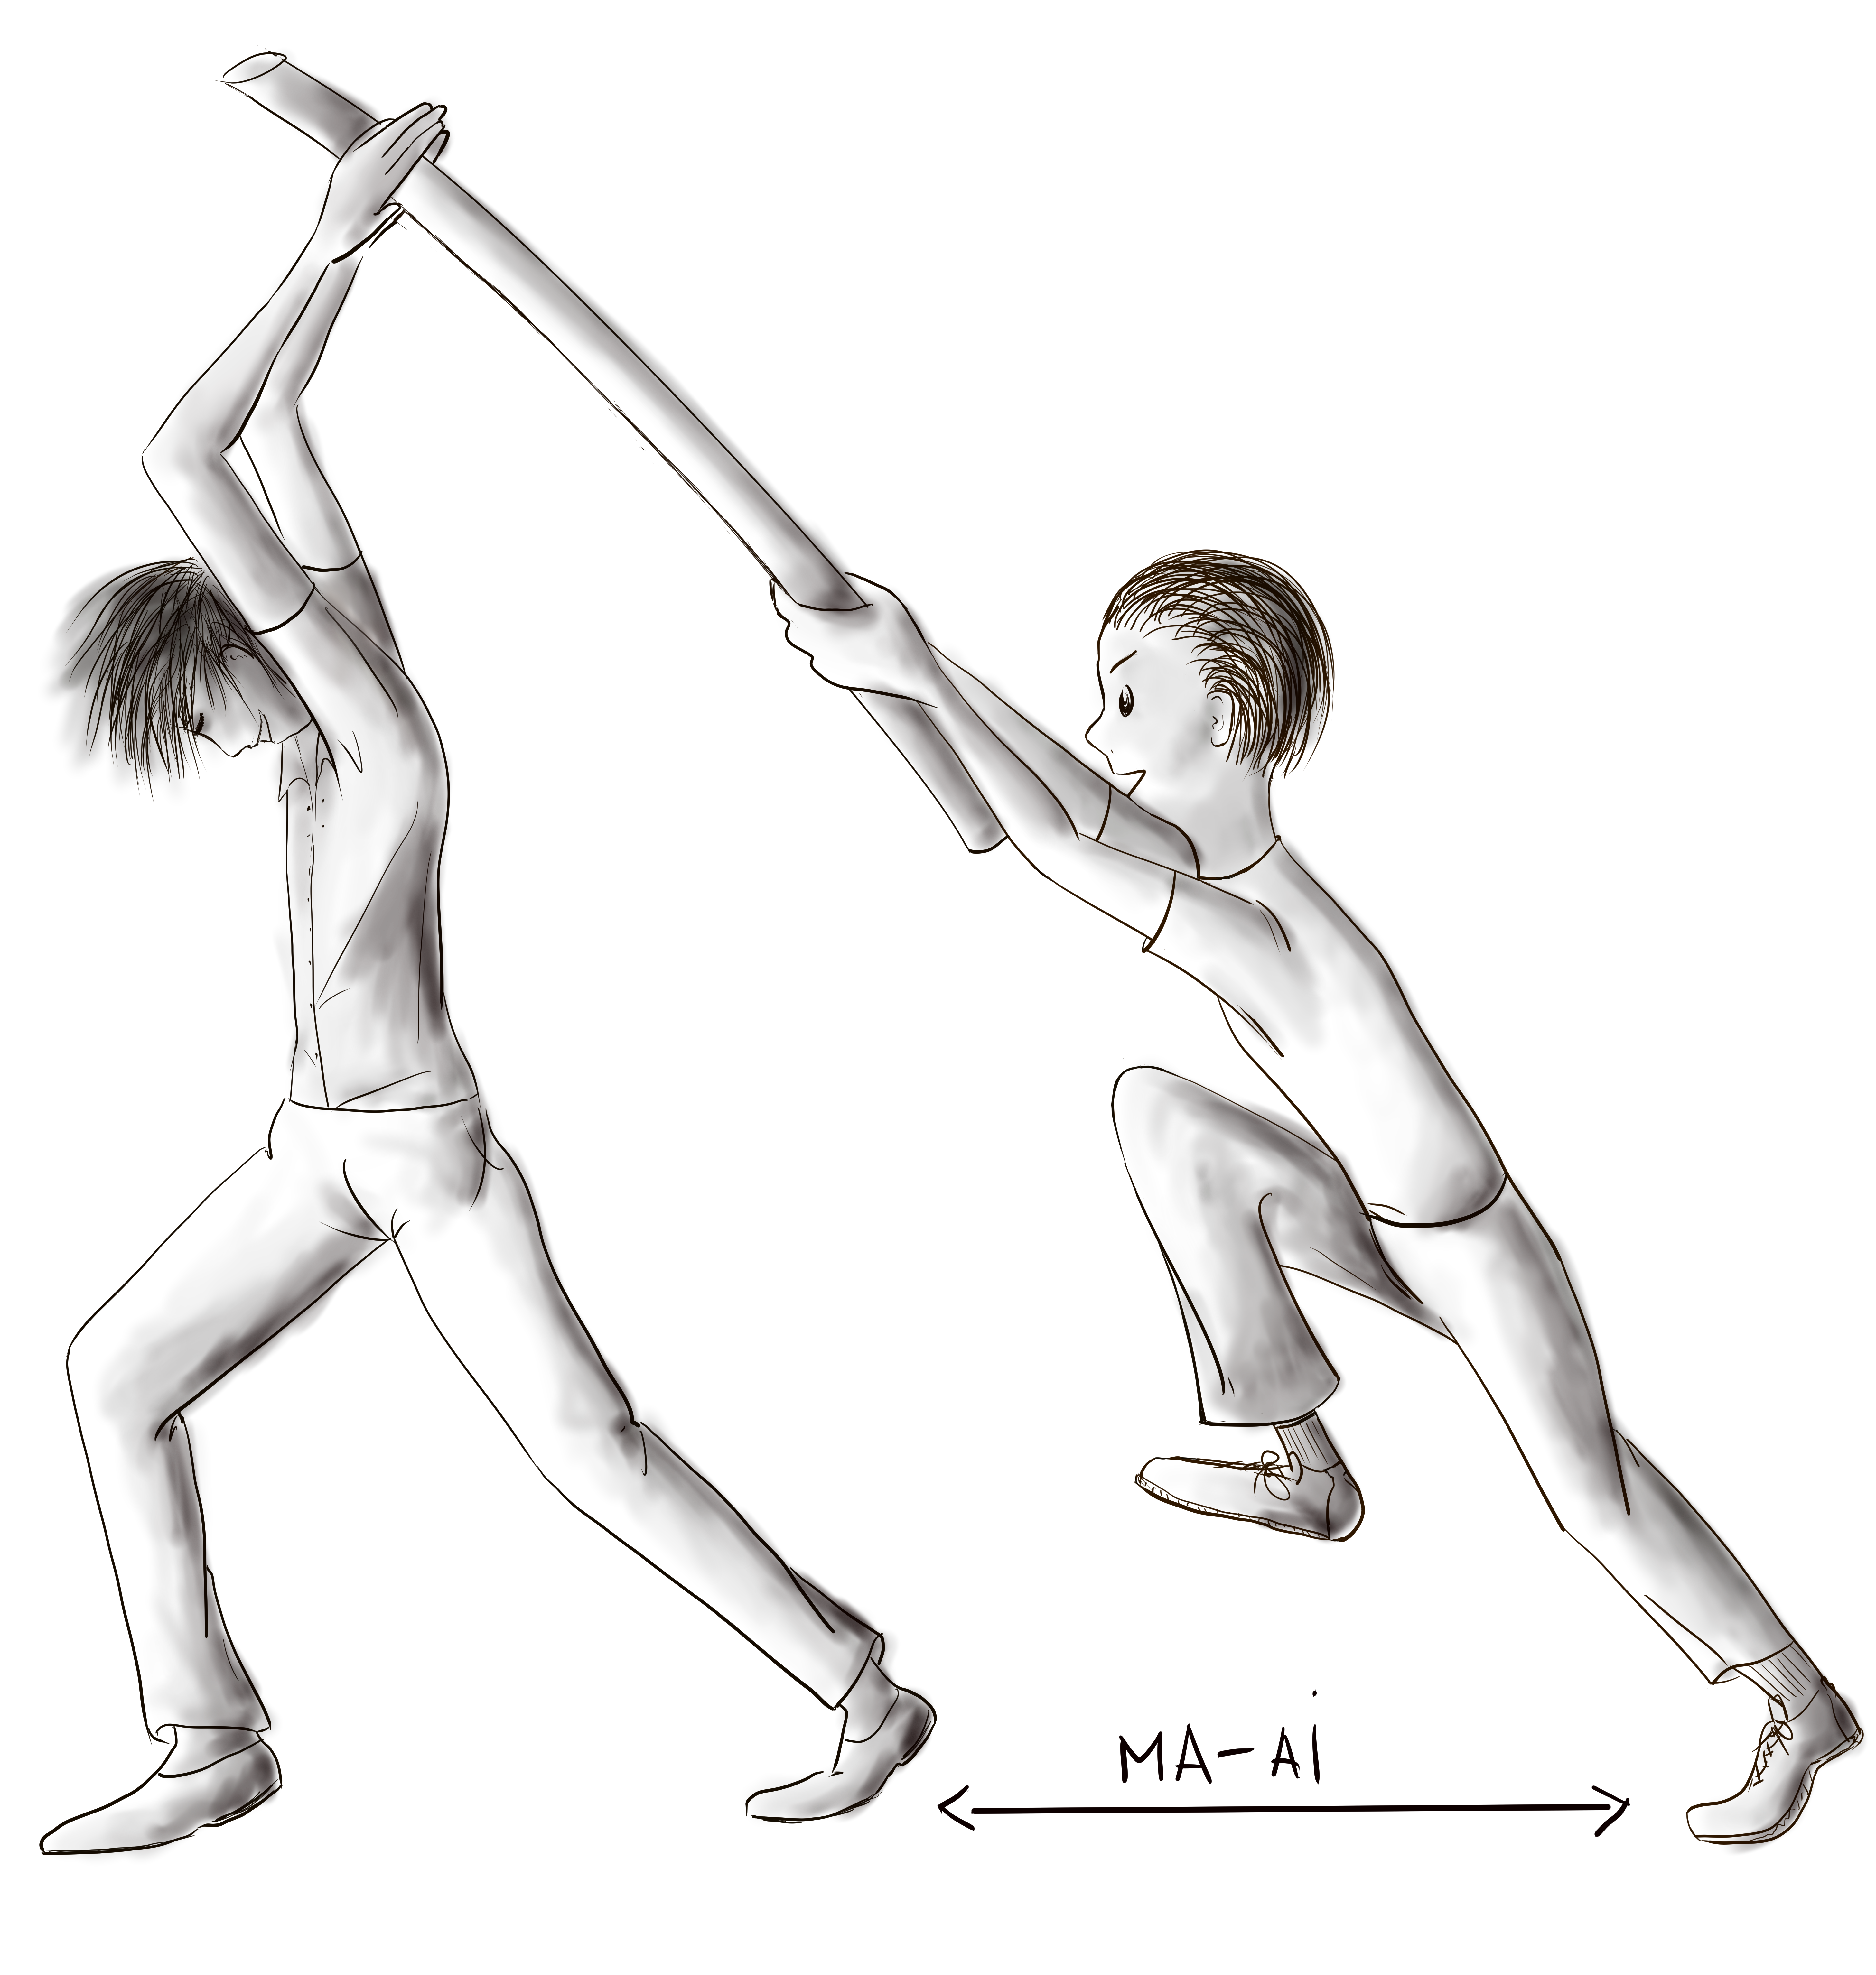
\includegraphics[width=0.6\linewidth]{media/ma ai senza sfondo.png}
\end{center}

\par\medskip
«Dai» gli dice. «Adesso aiutami. Prendi il pacco, Luca.»\\
«Ma questo? Dove lo hai preso?»\\
«Non lo so. Ha seguito Ipparchia.»\\
«E come si chiama?»\\
«Non lo so.»

\par\medskip
«Ecco, è scritto sul collare, Rocky.»

\par\medskip
Rocky lo guarda. Ha riconosciuto il suo nome.\\
«C’è un numero da chiamare?»\\
«Sì, è qui, guarda.»

\par\medskip
Passa qualche istante.\\
«Scusa, comunque c’è.»\\
«Bene, allora domani lo accompagneremo dai vigili. Ci penseranno loro. Portiamolo dentro e speriamo che per oggi non scappi.»\\
«Lo leghiamo?»

\par\medskip
Giovanni attende. Non risponde subito.\\
«No, prima la libertà.»

\par\medskip
Luca solleva il pacco e salgono per le scale antincendio. Poi un rumore improvviso.\\
«Attento!»

\par\medskip
Luca riprende l’equilibrio. La scala è senza parapetto e alcuni gradini sono bucati. Ma con un po’ di attenzione i due riescono a raggiungere la porta a finestra del primo piano.

\par\medskip
Ma un carrello della spesa carico di stracci e prodotti blocca l’entrata.

\par\medskip
Non è un carrello in buone condizioni. Mancano diverse sfere dai cuscinetti delle ruote, ma sarebbe comodo per portare la spesa dal supermercato. Ormai di carrelli non se ne trovano più.

\par\medskip
«Meglio salire al secondo.»\\
«Ci sono, le pulizie?»\\
«Mi sa di sì.»\\
«Ok, saliamo.»\\
«Ci segue anche Rocky?»\\
«Sì, è dietro Ippa.»\\
«Speriamo non facciano storie… già si lamentano di lei.»

\par\medskip
«Dovrebbero essere in aula 1. Se scendiamo dritti non lo vedranno neanche.»\\
«Hai ragione.»

\par\medskip
Giovanni rallenta il passo per assicurarsi del terreno sotto i piedi, perché non conosce bene la seconda rampa delle scale. Entrare al primo piano è molto più semplice, ma adesso le casalinghe stanno facendo le pulizie, e a memoria di convitto nessuno ha mai calpestato dove le casalinghe stanno pulendo.

\par\medskip
Sarebbe un errore irreparabile, perché significativo di ignoranza delle regole elementari di appartenenza a una comunità rispettabile. Basta riconoscere alcuni segnali elementari per non creare situazioni problematiche, e uno di questi è la presenza del carrello dei prodotti: un segnale universale di pulizia in corso. Impensabile spostarlo per passare. Essere civili si riconosce da queste attenzioni.
